\begin{frame}
	\frametitle{$\DPLL$ algorithms}

    \begin{center}
    	\onslide<1->{
   	\tikzstyle{vertex2} = [opacity = 0]
   	\tikzstyle{vertex3} = [opacity = 0]
    \tikzstyle{vertex4} = [opacity = 0]
   	\tikzstyle{vertex5} = [opacity = 0]
    \tikzstyle{vertex9} = [opacity = 0]
    \tikzstyle{vertex11} = [opacity = 0]
}
\only<2->{\tikzstyle{vertex2} = [opacity = 1]}
\only<3->{\tikzstyle{vertex3} = [opacity = 1]}
\only<4->{\tikzstyle{vertex4} = [opacity = 1]}
\only<5->{
  	\tikzstyle{vertex5} = [opacity = 1]
    \tikzstyle{vertex9} = [opacity = 1]
}

\tikzstyle{end} = [circle, minimum size = 0.6cm, draw, inner sep = 0.1pt]
            
\tikzstyle{level 1} = [level distance = 1.5cm, sibling distance = 5cm]
\tikzstyle{level 2} = [sibling distance = 2cm]
    
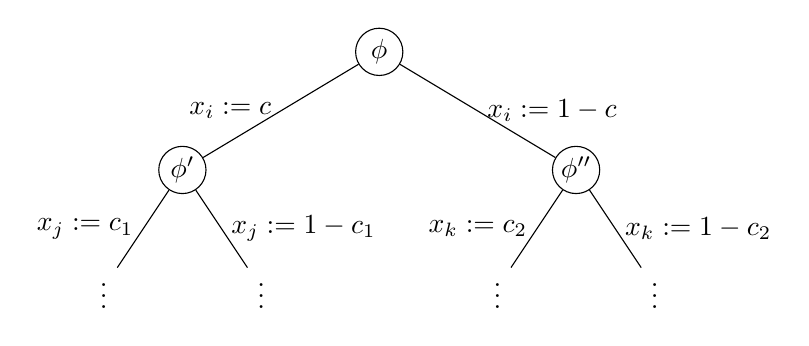
\begin{tikzpicture}[label distance = 8mm]
	\node [end] (z){$\phi$}
       	child [vertex2] {node [end] (b) {$\phi'$}
			child [vertex3]{
	           	node {$\vdots$}
                edge from parent
	  	        node[left] {$x_{j} := c_1$}
            }
		    child [vertex4]{
               	node {$\vdots$}
                edge from parent
	   	        node[right] {$x_{j} := 1 - c_1$}
            }
           	edge from parent
            node[left] {$x_{i} := c$}
        }
        child [vertex5] {node [end] (c) {$\phi''$}
           	child [vertex9]{
               	node {$\vdots$}
                edge from parent
	            node[left] {$x_{k} := c_2$}
            }
		    child [vertex9]{
               	node {$\vdots$}
                edge from parent
	            node[right] {$x_{k} := 1 - c_2$}
            }
            edge from parent
	   	    node[right] {$x_{i} := 1 - c$}
        };
\end{tikzpicture}
    
    \end{center}
    
	\pause
    \pause
    \pause
    \pause
    \pause

    The vertex is a leaf iff there is an empty clause in current formula.

\end{frame}


\begin{frame}
	\frametitle{Linear splitting tree (LST)}

    \begin{center}
    	\onslide<1->{
   	\tikzstyle{vertex2} = [opacity = 0]
   	\tikzstyle{vertex3} = [opacity = 0]
    \tikzstyle{vertex4} = [opacity = 0]
   	\tikzstyle{vertex5} = [opacity = 0]
    \tikzstyle{vertex9} = [opacity = 0]
    \tikzstyle{vertex11} = [opacity = 0]
}
\only<2->{\tikzstyle{vertex2} = [opacity = 1]}
\only<3->{\tikzstyle{vertex3} = [opacity = 1]}
\only<4->{\tikzstyle{vertex4} = [opacity = 1]}
\only<5->{
  	\tikzstyle{vertex5} = [opacity = 1]
    \tikzstyle{vertex9} = [opacity = 1]
}

\tikzstyle{end} = [circle, minimum size = 0.6cm, draw = black, inner sep = 0.1pt]
            
\tikzstyle{level 1} = [draw = black, level distance = 1.5cm, sibling distance = 5cm]
\tikzstyle{level 2} = [sibling distance = 2cm]
    
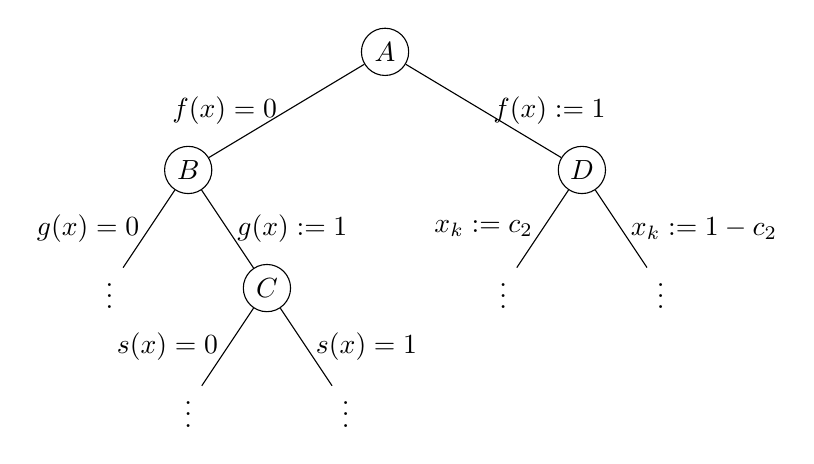
\begin{tikzpicture}[label distance=8mm]
	\node [end] (z){$A$}
		child [vertex2] {
    		node [end] (b) {$B$}
			child [vertex3]{
	           	node {$\vdots$}
                edge from parent
	  	        node[left] {$g(x) = 0$}
            }
		    child [vertex4]{
            	node[end] {$C$}
            	child [vertex4]{
            	   	node {$\vdots$}
            		edge from parent
	  	        	node[left] {$s(x) = 0$}
                }
                child [vertex4]{
            	   	node {$\vdots$}
            		edge from parent
	  	        	node[right] {$s(x) = 1$}
            	}
                edge from parent
	   	        node[right] {$g(x) := 1$}
            }
           	edge from parent
            node[left] {$f(x) = 0$}
        }
        child [vertex5] {
        	node [end] (c) {$D$}
           	child [vertex9]{
               	node {$\vdots$}
                edge from parent
	            node[left] {$x_{k} := c_2$}
            }
		    child [vertex9]{
               	node {$\vdots$}
                edge from parent
	            node[right] {$x_{k} := 1 - c_2$}
            }
            edge from parent
	   	    node[right] {$f(x) := 1$}
        };
\end{tikzpicture}
    
    \end{center}

    \vspace{0.1cm}
    
    \begin{minipage}{0.42\linewidth}
        \begin{itemize}
            \item<1-> $A := (\phi, \emptyset)$
	    	\item<2-> $B := (\phi, \{f(x)~=~0\})$
        \end{itemize}
    \end{minipage}
    \begin{minipage}{0.55\linewidth}
        \begin{itemize}
            \item<4-> $C := (\phi, \{f(x) = 0, g(x) = 1\})$
        	\item<5-> $D := (\phi, \{f(x) = 1\})$
        \end{itemize}
    \end{minipage}
    
	\pause
    \pause
    \pause
    \pause

\end{frame}


\begin{frame}
    \frametitle{Linear splitting trees (LST)}
    
	Solving CNF SAT using splitting by linear forms over $\mathbb{F}_2$.

    \begin{columns}[T]
        \begin{column}{4cm}
            \begin{enumerate}
                \item<1-> Degenerate leaf.
                \item<2-> Sat. assignment.
            	\item<3-> Contradiction with a clause.
            \end{enumerate}
        \end{column}
        \begin{column}{4cm}
            \begin{minipage}[c][.6\textheight][c]{\linewidth}
                \only<1>{\tikzstyle{end} = [circle, minimum size = 0.1cm, draw, inner sep = 0.1pt]
\tikzstyle{leaf} = [circle, minimum size = 0.6cm, draw, inner sep = 0.1pt, blue]
            
\tikzstyle{level 1}=[level distance = 1cm, sibling distance = 1cm]
\tikzstyle{level 2}=[level distance = 1.5cm, sibling distance = 1.5cm]
\tikzstyle{level 3}=[level distance = 1.5cm, sibling distance = 1.8cm]


    
\begin{tikzpicture}[label distance = 8mm]
	\node [end] (z){}
        child {
        	node[end] (b) {}
            child {
    			node {$\vdots$}
		        edge from parent
	    		node[left] {}
			}
		    child {
		        node[end] {}
                child {
                  	node {\alert{no sol.}}
                    edge from parent
                    node[left] {$y = 0$}
                }
                child {
        			node {$\vdots$}
		           	edge from parent
        		    node[right] {$y = 1$}
		        }
	            edge from parent
		        node[right] {$x + y = 1$}
            }
           	edge from parent
            node[left] {$x = 0$}
        }
        child {
        	node (b) {$\vdots$}
           	edge from parent
            node[right] {}
        };
\end{tikzpicture}

%%% Local Variables: 
%%% mode: latex
%%% TeX-master: t
%%% End: 
}
                \only<2>{\tikzstyle{end} = [circle, minimum size = 0.1cm, draw, inner sep = 0.1pt]
\tikzstyle{leaf} = [circle, minimum size = 0.6cm, draw, inner sep = 0.1pt, blue]
            
\tikzstyle{level 1}=[level distance = 1cm, sibling distance = 1cm]
\tikzstyle{level 2}=[level distance = 1.5cm, sibling distance = 1.5cm]
\tikzstyle{level 3}=[level distance = 1.5cm, sibling distance = 1.8cm]


    
\begin{tikzpicture}[label distance = 8mm]
	\node [end] (z){}
        child {
        	node[end] (b) {}
            child {
    			node {$\vdots$}
		        edge from parent
	    		node[left] {}
			}
		    child {
		        node[end] {}
                child {
        			node {$\vdots$}
		           	edge from parent
        		    node[left] {$z = 1$}
		        }
                child {
                  	node[blue] {\begin{tabular}{c} $x = 0$ \\ $y = 1$ \\ $z = 0$ \end{tabular}}
                    edge from parent
                    node[right] {$z = 0$}
                }
	            edge from parent
		        node[right] {$x + y = 1$}
            }
           	edge from parent
            node[left] {$x = 0$}
        }
        child {
        	node (b) {$\vdots$}
           	edge from parent
            node[right] {}
        };
\end{tikzpicture}

%%% Local Variables: 
%%% mode: latex
%%% TeX-master: t
%%% End: 
}
                \only<3>{\tikzstyle{end} = [circle, minimum size = 0.1cm, draw, inner sep = 0.1pt]
\tikzstyle{leaf} = [circle, minimum size = 0.6cm, draw, inner sep = 0.1pt, blue]
            
\tikzstyle{level 1}=[level distance = 1cm, sibling distance = 1cm]
\tikzstyle{level 2}=[level distance = 1.5cm, sibling distance = 1.5cm]
\tikzstyle{level 3}=[level distance = 1.5cm, sibling distance = 1.8cm]


    
\begin{tikzpicture}[label distance = 8mm]
	\node [end] (z){}
        child {
        	node[end] (b) {}
   		    child {
		        node {\alert{(*)}}
	            edge from parent
		        node[left] {$x + y = 0$}
            }
            child {
    			node {$\vdots$}
		        edge from parent
	    		node[right] {}
			}
           	edge from parent
            node[left] {$x = 0$}
        }
        child {
        	node (b) {$\vdots$}
           	edge from parent
            node[right] {}
        };
\end{tikzpicture}

%%% Local Variables: 
%%% mode: latex
%%% TeX-master: t
%%% End: 
}
        	\end{minipage}
        \end{column}
    \end{columns}
    
	$\Phi$ refutes $(x_1 \lor x_2 \dots \lor x_k)$ iff $\Phi \land (x_i = 1)$ is
    unsatisfiable $\forall i$.
\end{frame}



\begin{frame}
    \frametitle{Splitting over linear combinations}

	\begin{itemize}
		\item{} [Seto, Tamaki, 2011] Algorithm for Formula-SAT over the full binary
		    basis. For formulas of size $cn$ the algorithm runs $2^{(1 - \mu_c)n}$,
            where $\mu_c$ is a constant.
        \pause
		\item{} [Hirsch, Kulikov et al., 2015] Explicit construction of function with $3 \frac{1}{86}n$ circuit size.
	\end{itemize}    
\end{frame}